\chapter{Visualization Tools}
\label{cpt:tools}

The main contribution of this project is automatic methods for visualizing how a webcam scene varies, and for understanding the most important variations.  In most natural scenes, we notice changes in lighting, weather, and camera conditions which are interesting, but fail to describe the typical behavior of a scene.  The goal of these tools is to learn these variations and to point out changes independent of them.  PCA is a commonly used tool, and
captures a linear model of consistent image variations.  By analyzing the results of certain PCA setups, we can obtain important and interesting information.

\section{Setup}

The most obvious way to learn about scenes is to take the PCA decomposition of the entire webcam scene.  Unfortunately, our data-set is too large for this to be feasible, so we must limit our inputs.  Instead of taking a random subset of the images, if we can intelligently limit the images we give, we can get better inputs.

\subsection{Temporal Narrowing}

The AMOS data-set consists mostly of outdoor scenes.  These outdoor scenes vary significantly over the course of a day, going from night to day and back.  The change in lighting dominates all other changes across the scene, and causes many images to be completely dark.  Instead of wasting 

\subsection{Sky Mask}
In many outdoor scenes, even when narrowed to a particular time of day, the most difficult image
variation to characterize is the sky.  PCA has a difficult time learning changes in sunlight, clouds,
and other characteristics of the sky, even among a set of images of one time of day.  The variance in the sky dominates the PCA reconstruction, causing it to ignore information that is more interesting in this context.

Fortunately, it is fairly easy to learn which regions of an image are most affected by this.  In practice, a side effect of the rising and setting of the sun is that the first principal component of most scenes is the sky, as shown in \ref{fig:2skyPCA}.  By thresholding the values of this vector, we can effectively segment the sky from the rest of the image, as shown in \ref{fig:2skyMask}.

This simple mask allows PCA to focus on more interesting changes in the image, and most of the results that follow use a simple mask to ignore the sky regions of the images.  By setting all pixels in the sky to 0, we can effectively remove this difficulty.


\begin{figure}[ht]
	\centering
	\subfigure[]{
		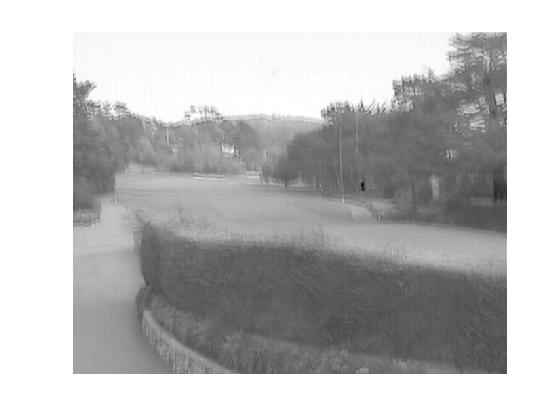
\includegraphics[width=0.45\textwidth]{figures/2skyPCA.jpg}
	\label{fig:2skyPCA}
	}
	\subfigure[]{
		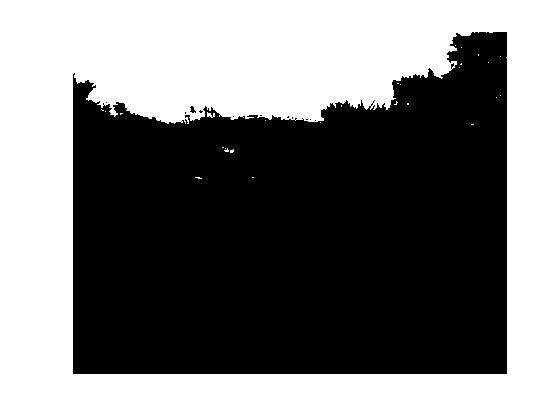
\includegraphics[width=0.45\textwidth]{figures/2skyMask.jpg}
	\label{fig:2skyMask}
	}
		\caption[Learning a sky mask for a webcam scene.]{Figure \ref{fig:2skyPCA} shows the first PCA component of a webcam scene.  By adding or subtracting this component, we control how dark or how light the sky is. Figure \ref{fig:2skyMask} shows that a simple thresholding of this image effectively segments the sky from the rest of the image.}
		
\end{figure}\subsection{Gradient Image}

Webcam images are very high-dimensional - a typical 320 x 240 gray scale image has 76,800 pixels, each of
which is a value from 0 to 255.  One way to simplify this space without changing the size of the image is to look at the gradient magnitude images of a scene.  

The x and y derivatives of an image are defined as $I_x(x,y) = I(x,y)-I(x-1,y)$ and $I_y(x,y) = I(x,y)-I(x,y-1)$ where the function $I(x,y)$ describes the intensities of an image's pixels.  Once we have calculated the derivative images, we define the gradient magnitude of an image to be $G(x,y) = I_x(x,y)^2 + I_y(x,y)^2$.

The gradient magnitude image highlights edges in an image, as they are image locations where pixel values differ greatly from their neighbors.  By performing PCA on the gradient magnitude images, we tend to ignore the potentially noisy surfaces of objects, and instead focus on the locations of the objects.  Figure \ref{fig:carsNoGradient} and Figure\ref{fig:carsGradient} show the edges of an interesting webcam image highlighted in a gradient magnitude image.


\begin{figure}[ht]
	\centering
	\subfigure[]{
		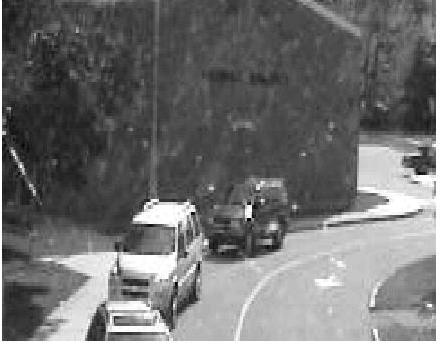
\includegraphics[width=0.45\textwidth]{figures/194cars.jpg}
	\label{fig:carsNoGradient}
	}
	\subfigure[]{
		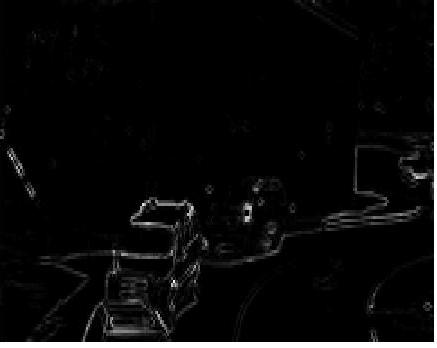
\includegraphics[width=0.45\textwidth]{figures/194carsGradient.jpg}
	\label{fig:carsGradient}
	}
		\caption[Focusing on object edges with gradient magnitude images.]{Figure \ref{fig:carsNoGradient} shows a grayscale webcam image. Figure \ref{fig:carsGradient} shows the gradient magnitude image of that frame.  Notice the noise is mostly removed and the edges are highlighted.}
\end{figure}

\section{Visualizations}

In this section, we present several tools to visualize the webcam scene based on criteria we will discuss in the next section.

\begin{figure}
	\centering
	\subfigure[]{
		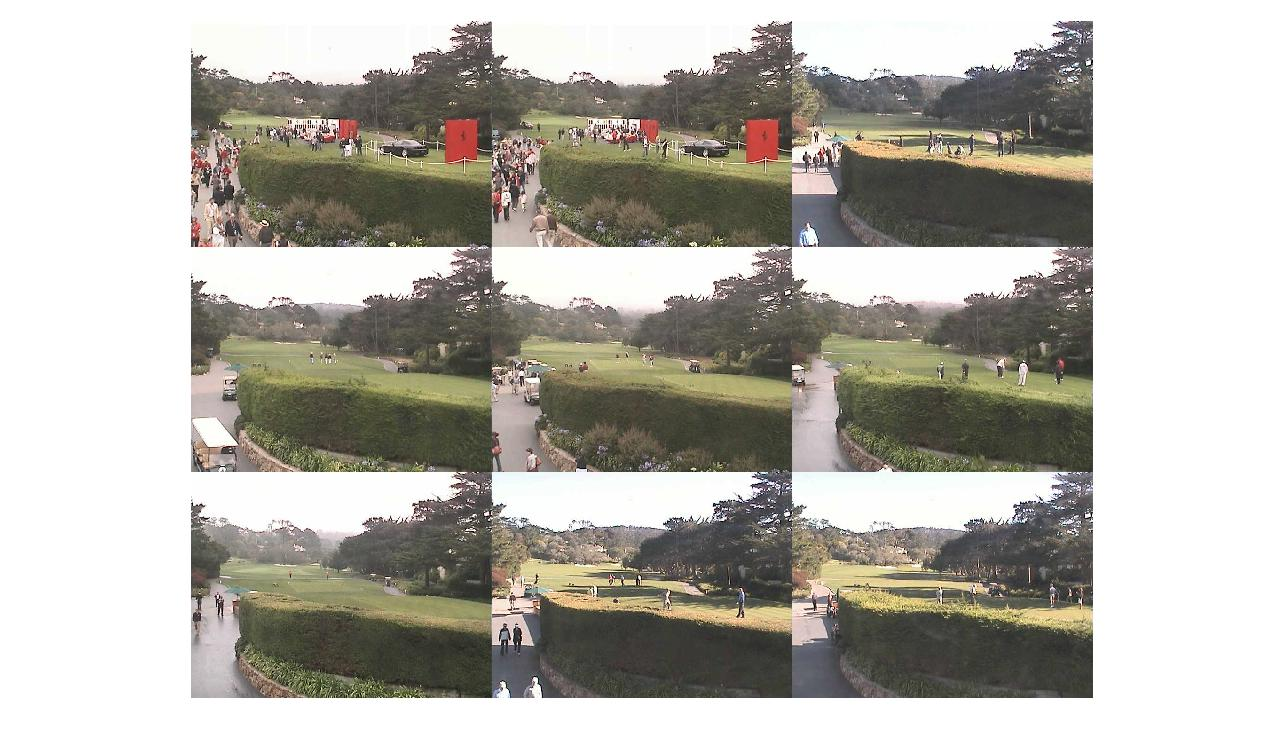
\includegraphics[width=1\textwidth]{figures/golfMontageNaive.jpg}
	\label{fig:golfMontageNaive}
	}
	\subfigure[]{
		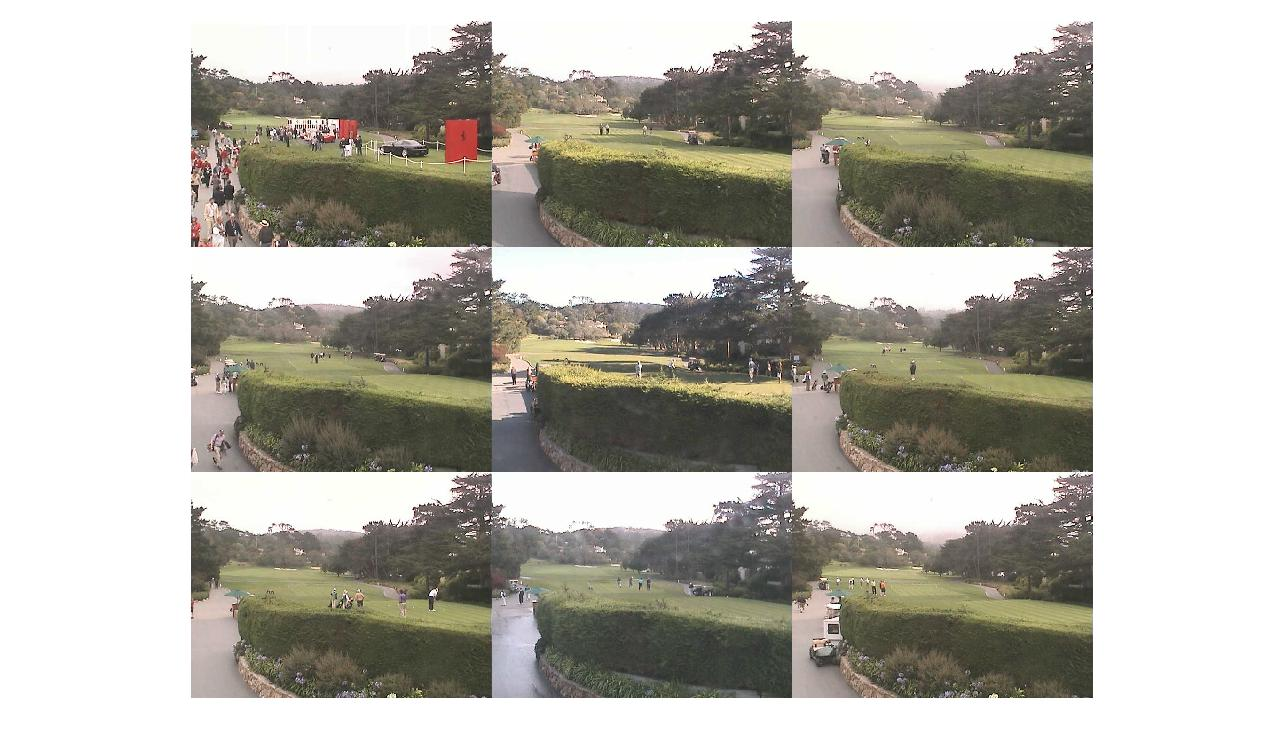
\includegraphics[width=1\textwidth]{figures/golfMontageSmart.jpg}
	\label{fig:golfMontageSmart}
	}
		\caption[Image montage techniques.]{Figure \ref{fig:golfMontageNaive} shows a montage of interesting images from a golf course webcam. Figure \ref{fig:golfMontageSmart} shows a montage of interesting images of the same scene, but attempts to omit similar images.}
\end{figure}

\subsection{Image Montage}

The simplest way to visualize a webcam scene is to view a montage of several images from that scene.  We can easily sort the images along some dimension, and then show the $n$ images with the highest values in that dimension.  Figure \ref{fig:golfMontageNaive} Is an example montage of several interesting images from a webcam scene.

\subsection{Well-Separated Set Montage}

In several of these montages, we notice that many of the most unusual images are similar to each other.  This presents the problem of finding unusual images that are different from the images we have already chosen.

A simple but effective algorithm for this problem uses the L2 norm in image space.  If we consider an image as a vector of pixel intensities, such as $v = \{v_1, ..., v_m\}$, the L2 norm of two images $v$ and $u$ is $$L2\_norm(v,u) = \sqrt{\sum_{i=1}^m{(v_i-u_i)^2}}$$  Given a large set of unusual images $\{x_1, ..., x_n\}$, we compute a distance matrix $D$ where $D_{i,j} = L2\_norm(x_i, x_j).$  Now we iteratively find unusual images by choosing the image that has the largest distance from all of the images we have chosen so far.  Specifically, for each remaining image calculate its distance to our set of exemplars, and choose the image whose distance is the smallest.  We define the distance of an image $x_0$ to a set of exemplars $\{x_1, ..., x_n\}$ as $$d = \min_i(D(x_0, x_i))$$In this way, on each iteration, we pick the image that is least likely to be similar to an image we have already selected.  We have found that a good way to seed this process is choosing the image with the highest unusualness score as our first exemplar.  \ref{fig:golfMontageSmart} shows how similar images are omitted by viewing results in this way.

\subsection{Two-dimensional Explorer}


Using a simple GUI, we can explore a webcam scene in two dimensions.  The GUI, shown in \ref{fig:2dGui}, displays a a plot of image scores for two different criteria, and displays the image corresponding to a mouseovered datapoint.  Using this GUI, it is possible to see which criterias are related and which are not, as well as makes it easier to learn how the criteria effects the scene. [I don't really know what to say in this section].

\begin{figure}[ht]
	\centering
		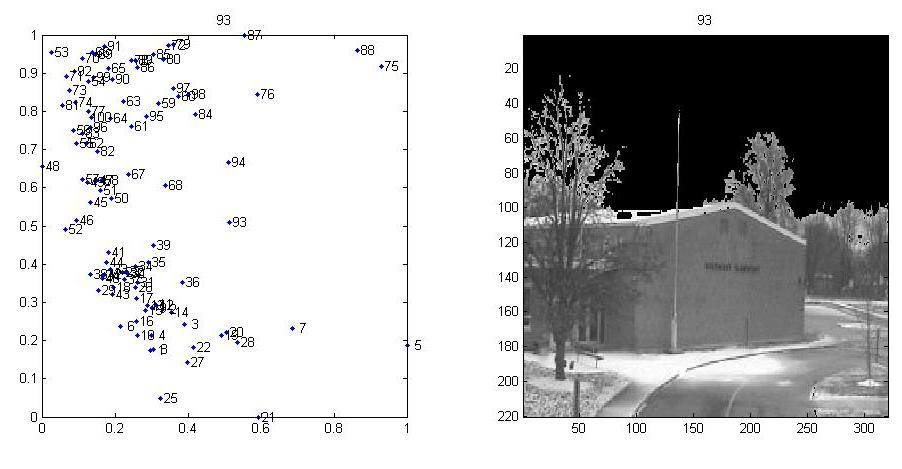
\includegraphics[width=1\textwidth]{figures/2dGui.jpg}
	\label{fig:2dGui}
	
		\caption[Exploring 2D image space using a simple GUI.]{Figure \ref{fig:2dGui} shows a webcam scene displayed using the 2D GUI.}
\end{figure}


\section{Characteristics of Image Residuals}

Once webcam scenes are projected onto a PCA basis, there are many different ways to analyze the results.  In this section, we will present several different criteria for evaluating this appearance model of a scene, the meaning behind each criteria, and results.

[I don't love the term criteria, but I think it encapsulates the idea of this section...]

\subsection{PCA coefficient vector magnitude}

\begin{figure}
	\centering
	\subfigure[]{
		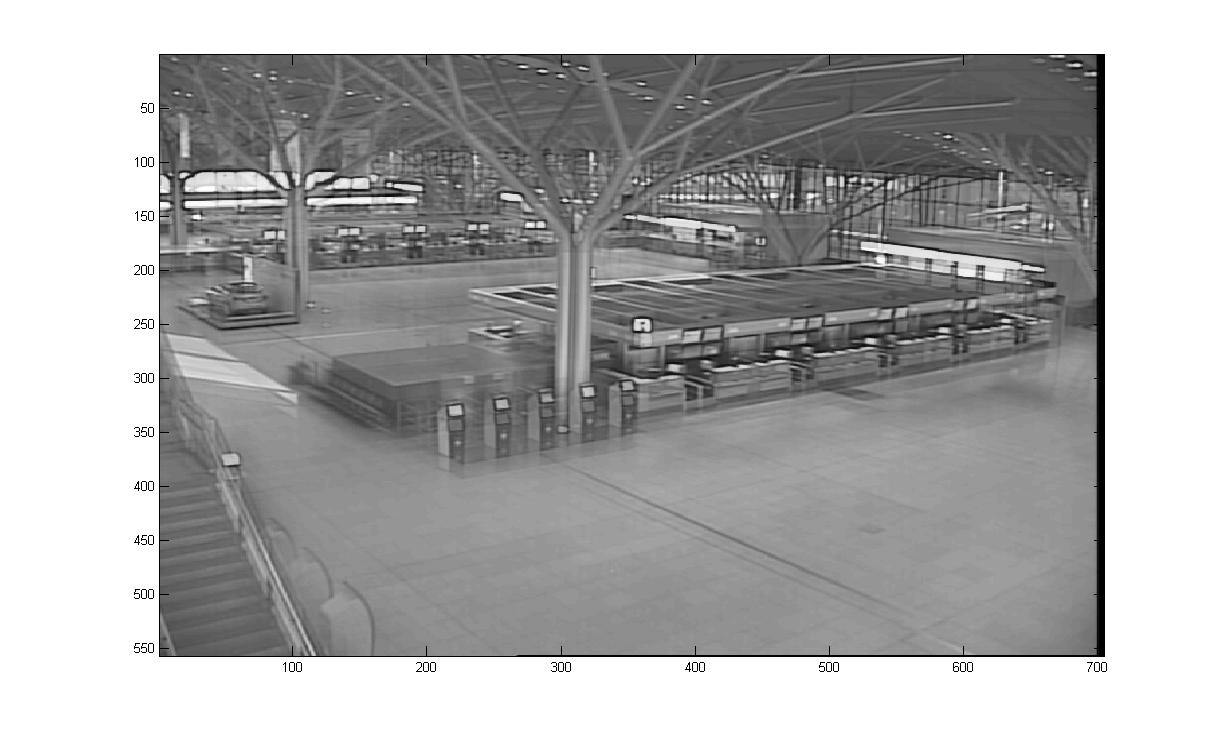
\includegraphics[width=.8\textwidth]{figures/vectorMagnitudeMean.jpg}
	\label{fig:vectorMagnitudeMean}
	}
	\subfigure[]{
		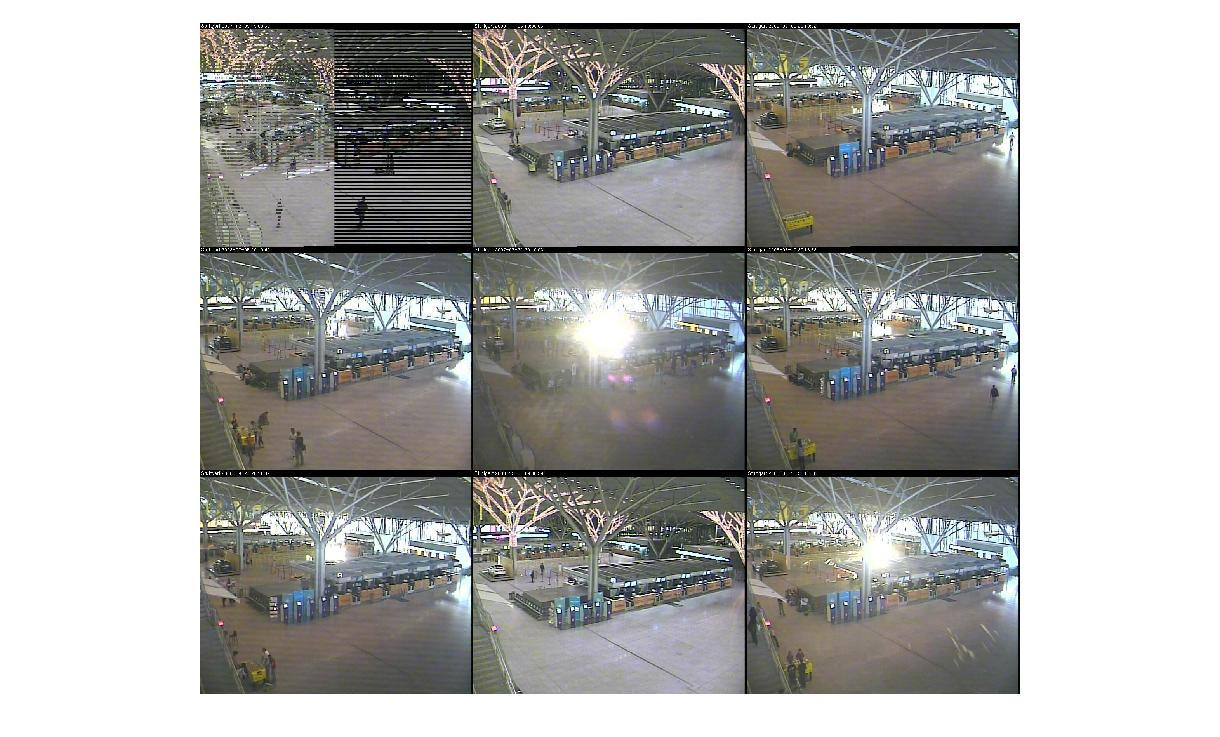
\includegraphics[width=1\textwidth]{figures/vectorMagnitudeMontage.jpg}
	\label{fig:vectorMagnitudeMontage}
	}
		\caption[Criteria: Gradient Magnitude.]{Figure \ref{fig:vectorMagnitudeMean} shows the mean image of an airport webcam scene. Figure \ref{fig:vectorMagnitudeMontage} shows several images found using this technique that are far from the mean.}
\end{figure}

For each image in a scene, PCA gives a vector of coefficients that correspond to the best linear combination of basis images to reconstruct that image.  From this vector, we can assign each image a score equal to the magnitude of this vector.  For a vector $v = (v_0, v_1, ..., v_n)$, the vector magnitude is $$||v||=\sqrt{\sum_{i=0}^nv_i^2}$$This effectively gives us a measure for how far from the mean image in our basis space each image is.  Figure \ref{fig:vectorMagnitudeMean} shows the mean image of a webcam scene and Figure \ref{fig:vectorMagnitudeMontage} shows several images from that webcam scene that are especially far from the mean.



\subsection{Residual Error}

Given an image and a PCA basis, we can project the image onto the basis and see how well we can reconstruct the image.

\begin{figure}
	\centering
		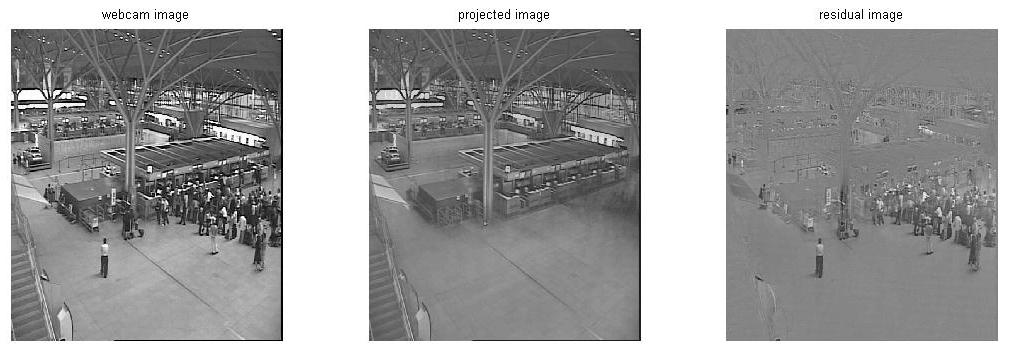
\includegraphics[width=1\textwidth]{figures/residualReconstruction.jpg}
	\label{fig:residualReconstruction}
	
		\caption[Residual Reconstruction.]{Figure \ref{fig:2dGui} show a webcam scene image, the reconstruction of that image from a PCA basis, and the residual image.}
\end{figure}

[Figure of subplot with image, reconstruction, and residual]

\begin{figure}
	\centering
		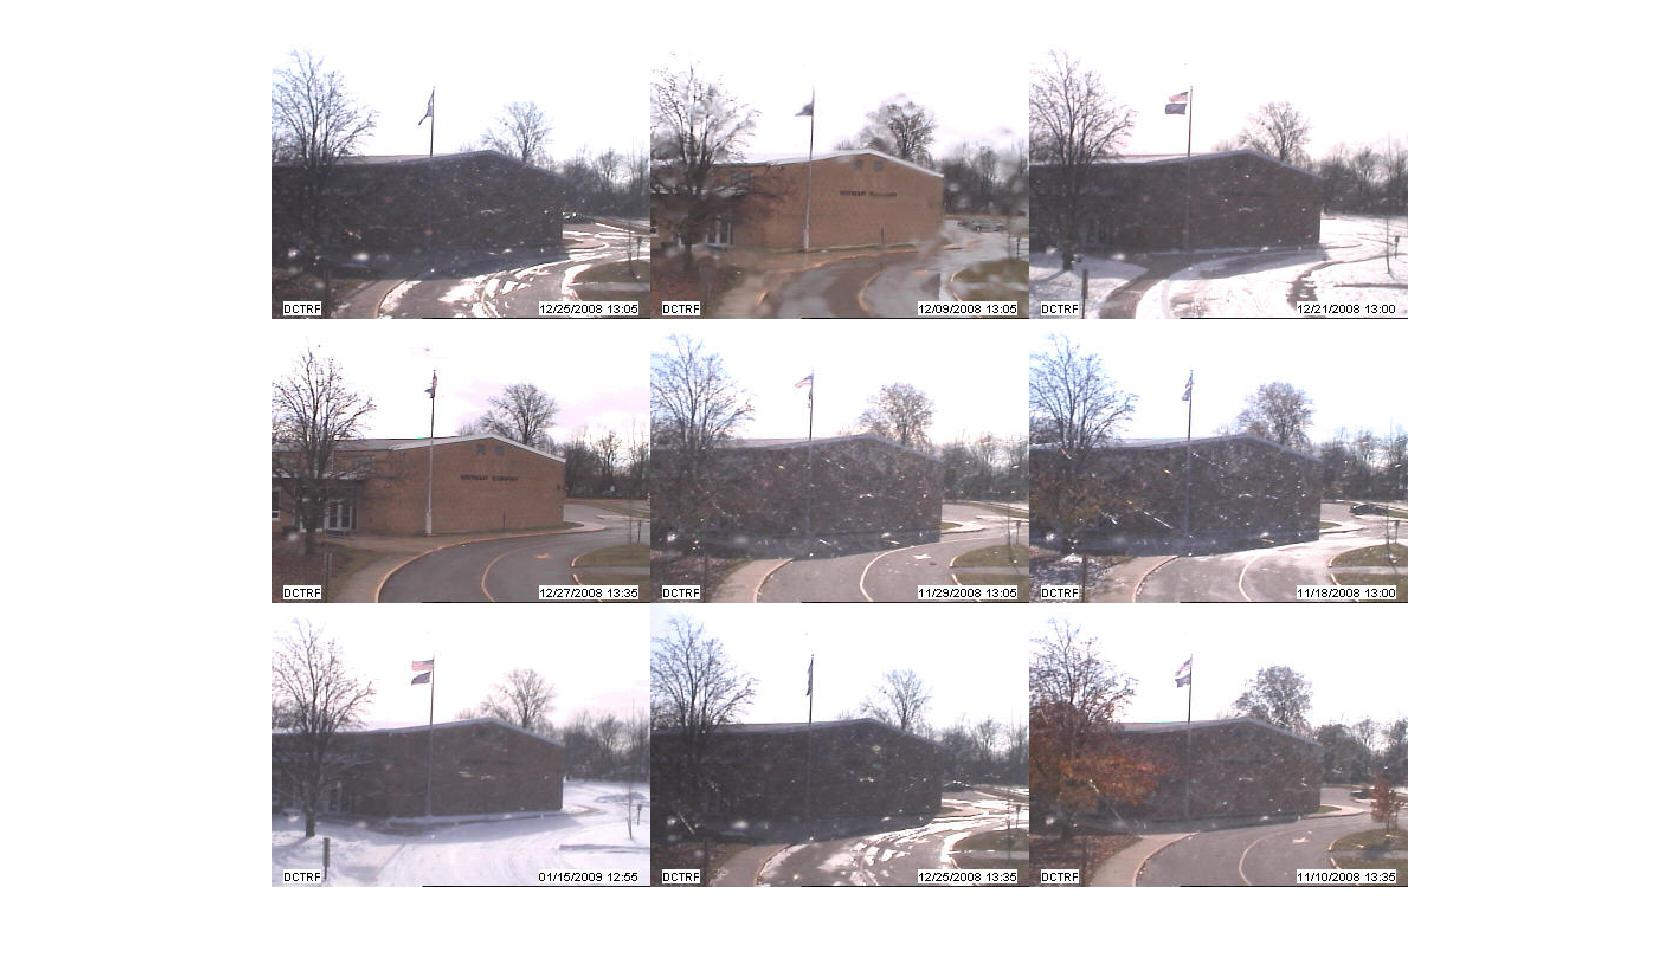
\includegraphics[width=1\textwidth]{figures/residualSSDmontage.jpg}
	\label{fig:residualSSDmontage}
	
		\caption[Residual SSD Montage.]{Figure \ref{fig:residualSSDmontage} show a webcam scene image, the reconstruction of that image from a PCA basis, and the residual image.}
\end{figure}

[figure of montage sorted be residualSSD, showing some noisy images and some with real foreground objects]


\subsection{Variance Model}

We can estimate the variance image of a webcam scene as the average of the square of each residual image.  This image gives a good summary as to where most activity occurs in a webcam scene.  Several examples are shown in Figure \ref{fig:severalVarianceImages}.

\begin{figure}
	\centering
		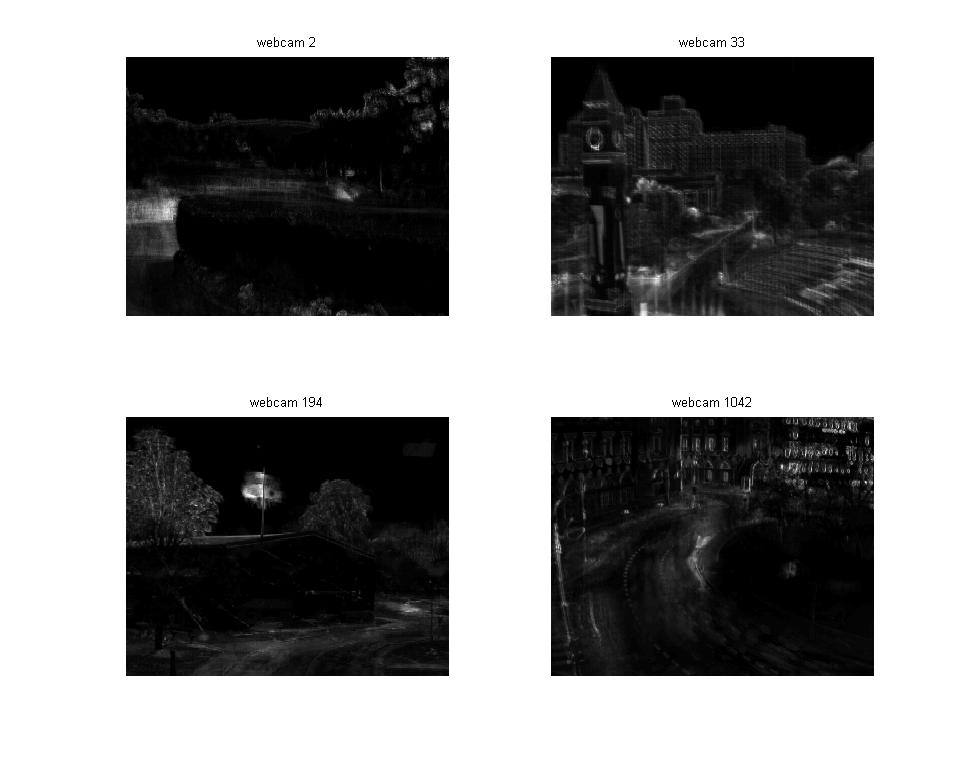
\includegraphics[width=1\textwidth]{figures/severalVarianceImages.jpg}
	\label{fig:severalVarianceImages}
	
		\caption[Several variance images.]{Figure \ref{fig:severalVarianceImages} shows estimated variance images from several webcam scenes.}
\end{figure}

One we have this variance image, we can attempt to isolate independent pixels in a z-score image.  We define our z-score image as $$Z(x,y) = \frac{R(x,y)} { V(x,y)}$$ where $R(x,y)$ is the residual value of the pixel and $V(x,y)$ is the variance value of the pixel.  By summing the per pixel z-score for an particular image, we can infer how atypical the residual of that image is.  Figure \ref{fig:residualZScoreMontage} shows several images that contain atypical objects.  Such a tool can be used to quickly highlight unusual behavior in a scene.

\begin{figure}
	\centering
		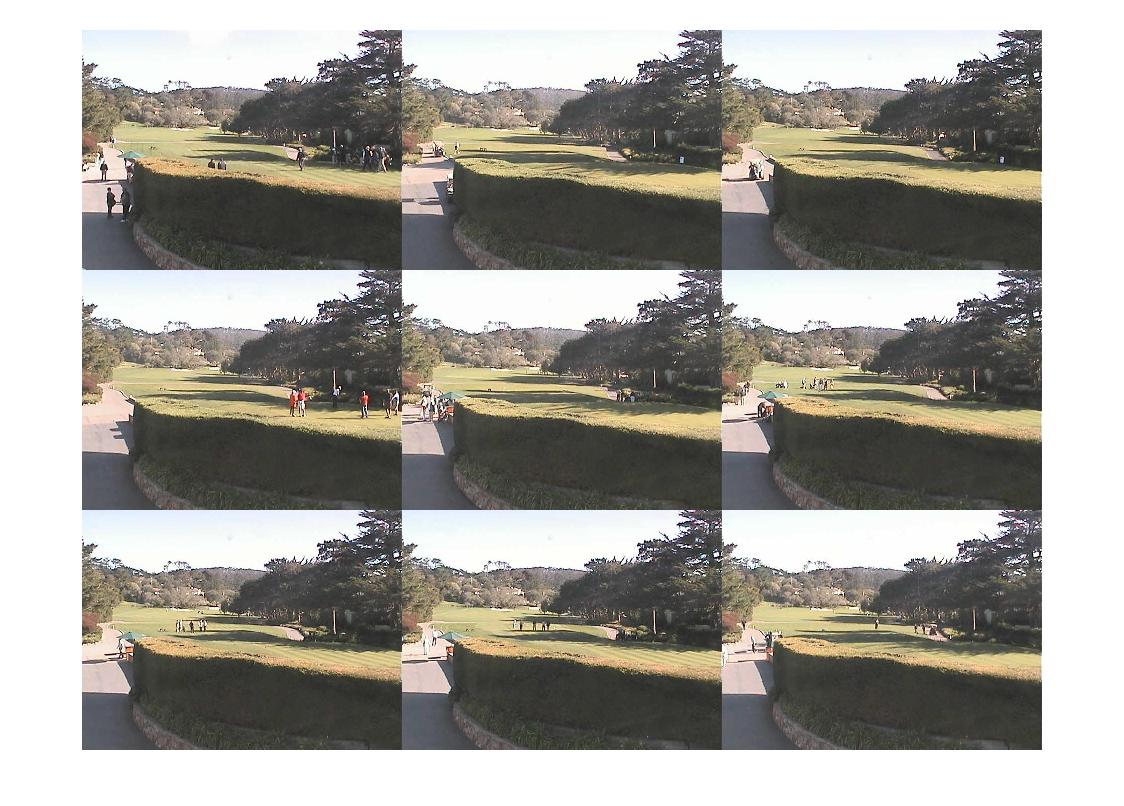
\includegraphics[width=1\textwidth]{figures/residualZScoreMontage.jpg}
	\label{fig:residualZScoreMontage}
	
		\caption[Z-Score Montage.]{Figure \ref{fig:residualZScoreMontage} shows several images from the same scene as \ref{fig:residualSSDmontage}, but with more atypical objects.}
\end{figure}





\subsection{Statistical Distribution of Residual Images}

We can also try to learn about an image reconstruction by treating its residual image as samples from an 
underlying probability density function.  If image deviations are due mostly to noise, we predict that these deviations will be normally distributed, but as shown in \ref{fig:severalHists}, this is not always the case.  We have found that these distributions vary in the same way as webcam scenes, and analyzing them in the right way tells an interesting story.


\begin{figure}
	\centering
		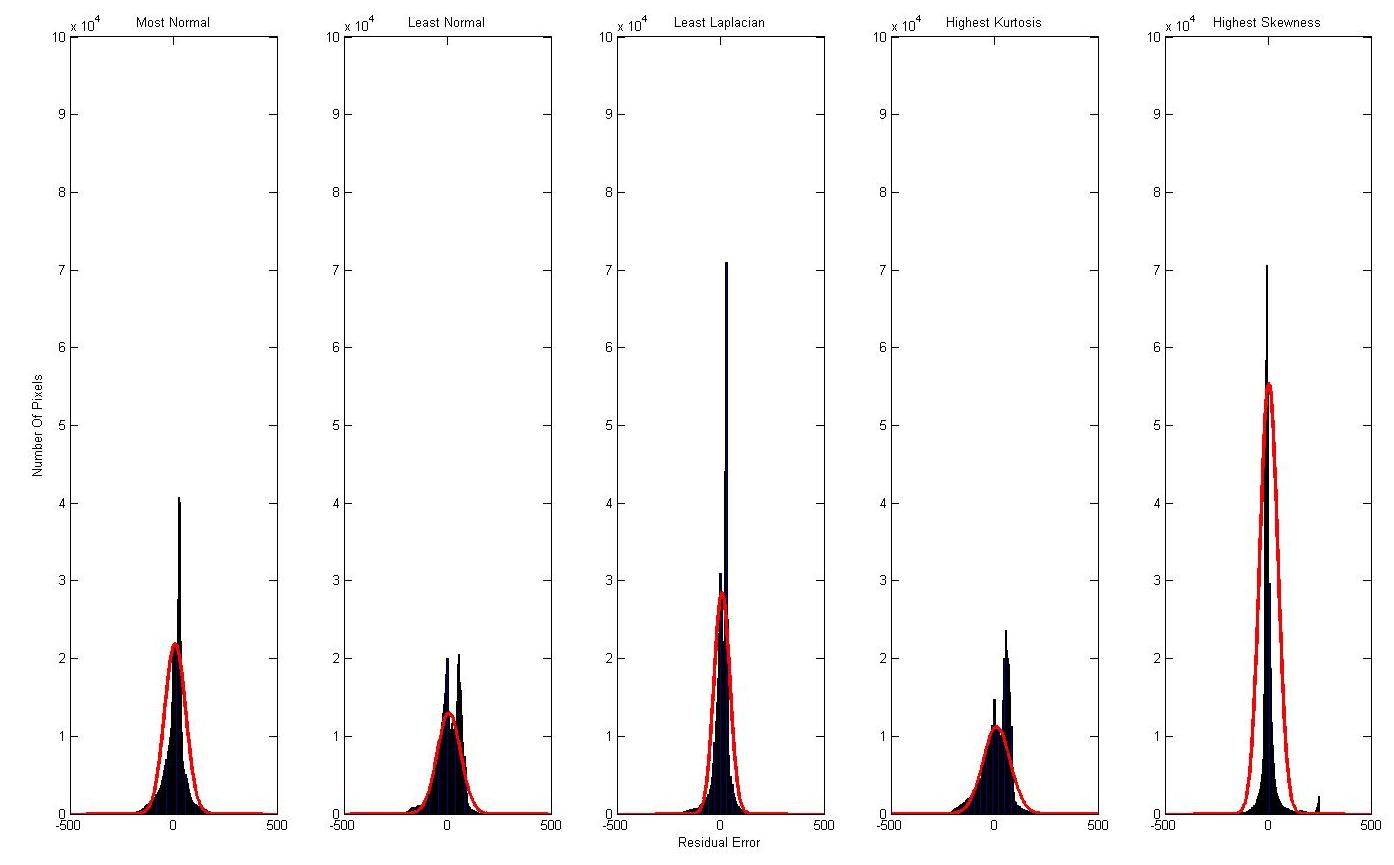
\includegraphics[width=1\textwidth]{figures/severalHists2.jpg}
	\label{fig:severalHists}
	
		\caption[Several residual image histograms.]{Several residual image histograms and the the best approximation of a normal distribution fitting the data.}
\end{figure}



\begin{figure}
	\centering
	\subfigure[]{
		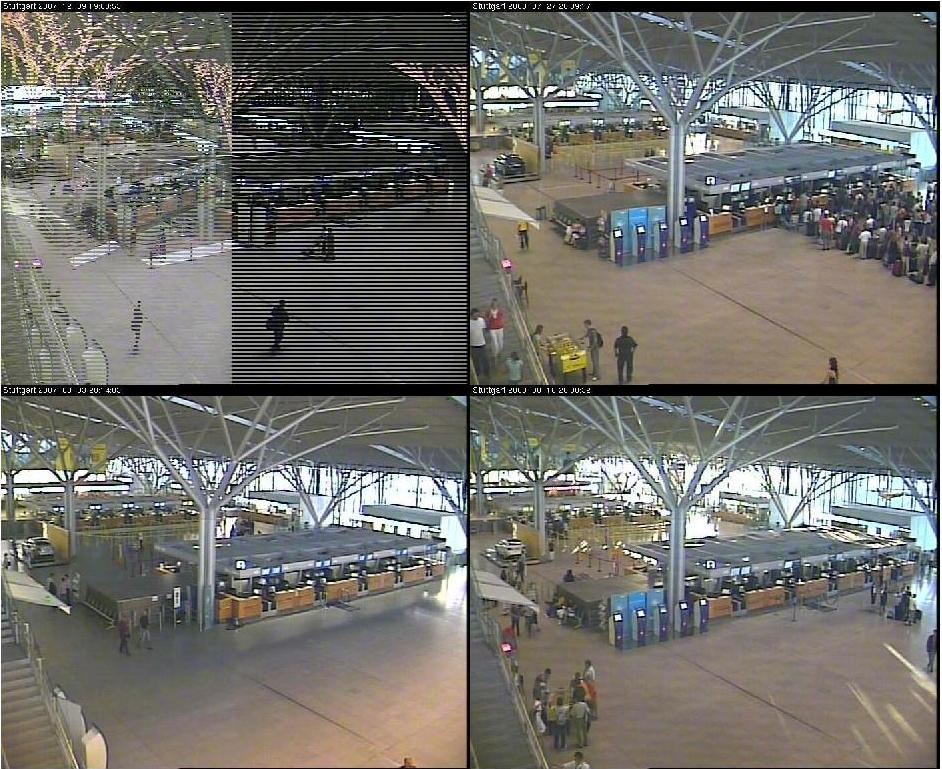
\includegraphics[width=.6\textwidth]{figures/leastNormal.jpg}
	\label{fig:leastNormal}
	}
	
	\subfigure[]{
		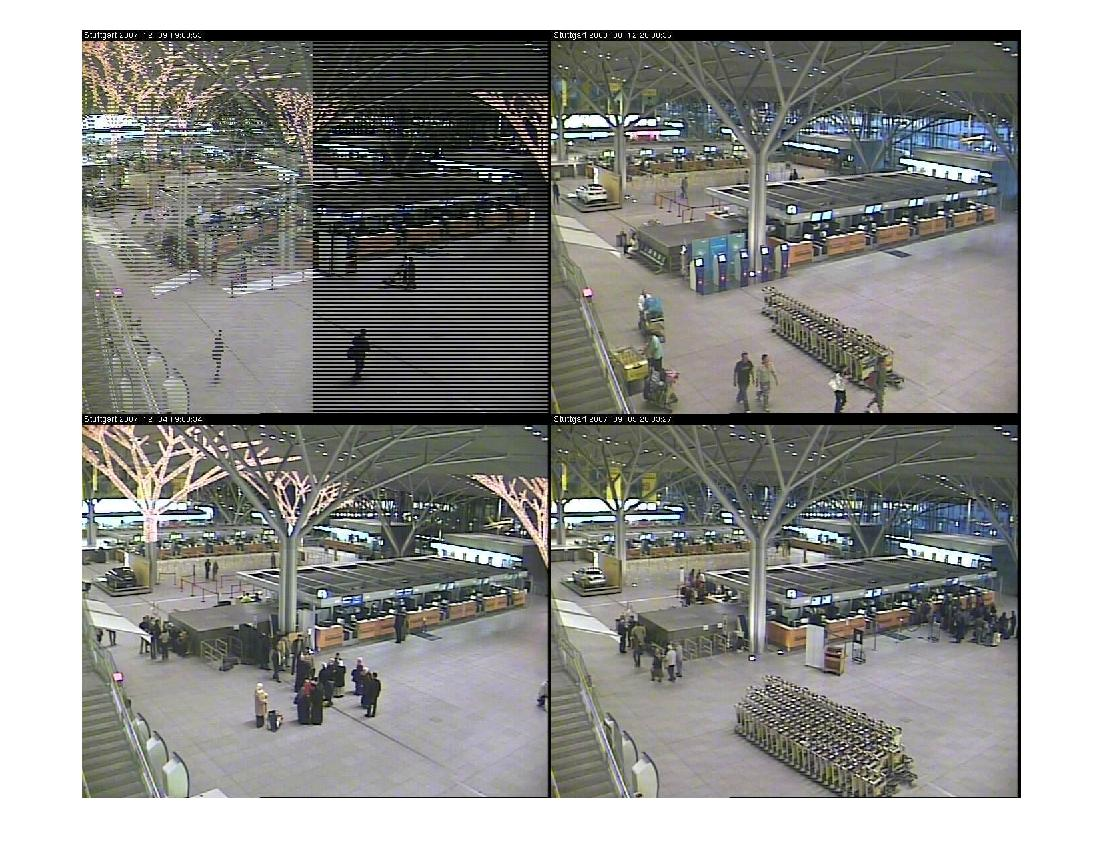
\includegraphics[width=.6\textwidth]{figures/leastLaplacian.jpg}
	\label{fig:leastLaplacian}
	}
	
			\caption[Least Gaussian and Least Laplacian Images.]{Figure \ref{fig:leastNormal} shows a montage of interesting images from an airport scene that were labeled very non-guassian. Figure \ref{fig:leastLaplacian} shows a montage of interesting images from an airport scene that were labeled very non-laplacian.}
\end{figure}



\begin{enumerate}
\item{\textbf{Gaussian Likelihood}}

The most obvious way to do this is to treat each residual image pixel as a sample from a normal distribution.  We can easily estimate the mean and variance of this PDF and then, for each residual value, use the normal distribution equation 

$$f(x|\mu,\sigma)=\frac{1}{\sigma\sqrt{2\pi}}e^{\frac{(x-\mu)^2}{2\sigma^2}}$$

 


\item{\textbf{Laplacian Likelihood}}

Many of the residual images have a majority of pixels that are very close zero.  This causes the histogram to look very similar to a laplacian distribution.

$$f(x|\mu,\beta)=\frac{1}{2\beta}e^{\frac{-|x-\mu|}{\beta}}$$

\item{\textbf{Kurtosis}}

The kurtosis of a real-valued random variable is a measure of its peakedness.  Larger values of kurtosis means more variance is due to less frequent extreme deviations rather than frequent less extreme deviations.  It is defined as $$\gamma_2=\frac{\mu_4}{\sigma^4}$$ where $\mu_4$ is the fourth moment about the mean and $\sigma^4$ is the estimated standard deviation to the fourth power.  For a function $f(x)$, the $k^{th}$ moment about the mean is defined as 

$$\mu_k = \int_{-\infty}^{\infty}{(x-\mu)^kf(x)dx}$$

We can use this measure 

\item{\textbf{Skewness}}

The skewness of a random variable is a measure of asymmetry.  Higher skewness values mean deviations on one side of the mean do not have corresponding deviations on the other side.  It is defined as $$\gamma_1=\frac{\mu_3}{\sigma^3}$$ where $\mu_3$ is the third moment about the mean and $\sigma^3$ is the cube of the standard deviation.

This measure can be used


\end{enumerate}


